\chapter{Almacenamiento de datos }
El almacenamiento de datos es un tema muy importante dentro de los m\'etodos num\'ericos, ya que es necesario tener un computador capaz de almacenar y resolver r\'apidamente los sistemas.

\section{Formas de matrices}
Alguanas ocaciones los sistemas de soluci\'on son muy grandes lo que implica un gran espacio de almancenamiento y esto puede provocar que la velocidad de soluci\'on no sea tan buena. Es por eso que se implementan t\'ecnicas de reducci\'on matricial, para acelerar el tiempo de soluci\'on de sistemas robustos sin afectar el resultado.\\
Para esto, la forma de la matriz influye por la manera en que fueron enumerados cada uno de los elementos.

\begin{center}
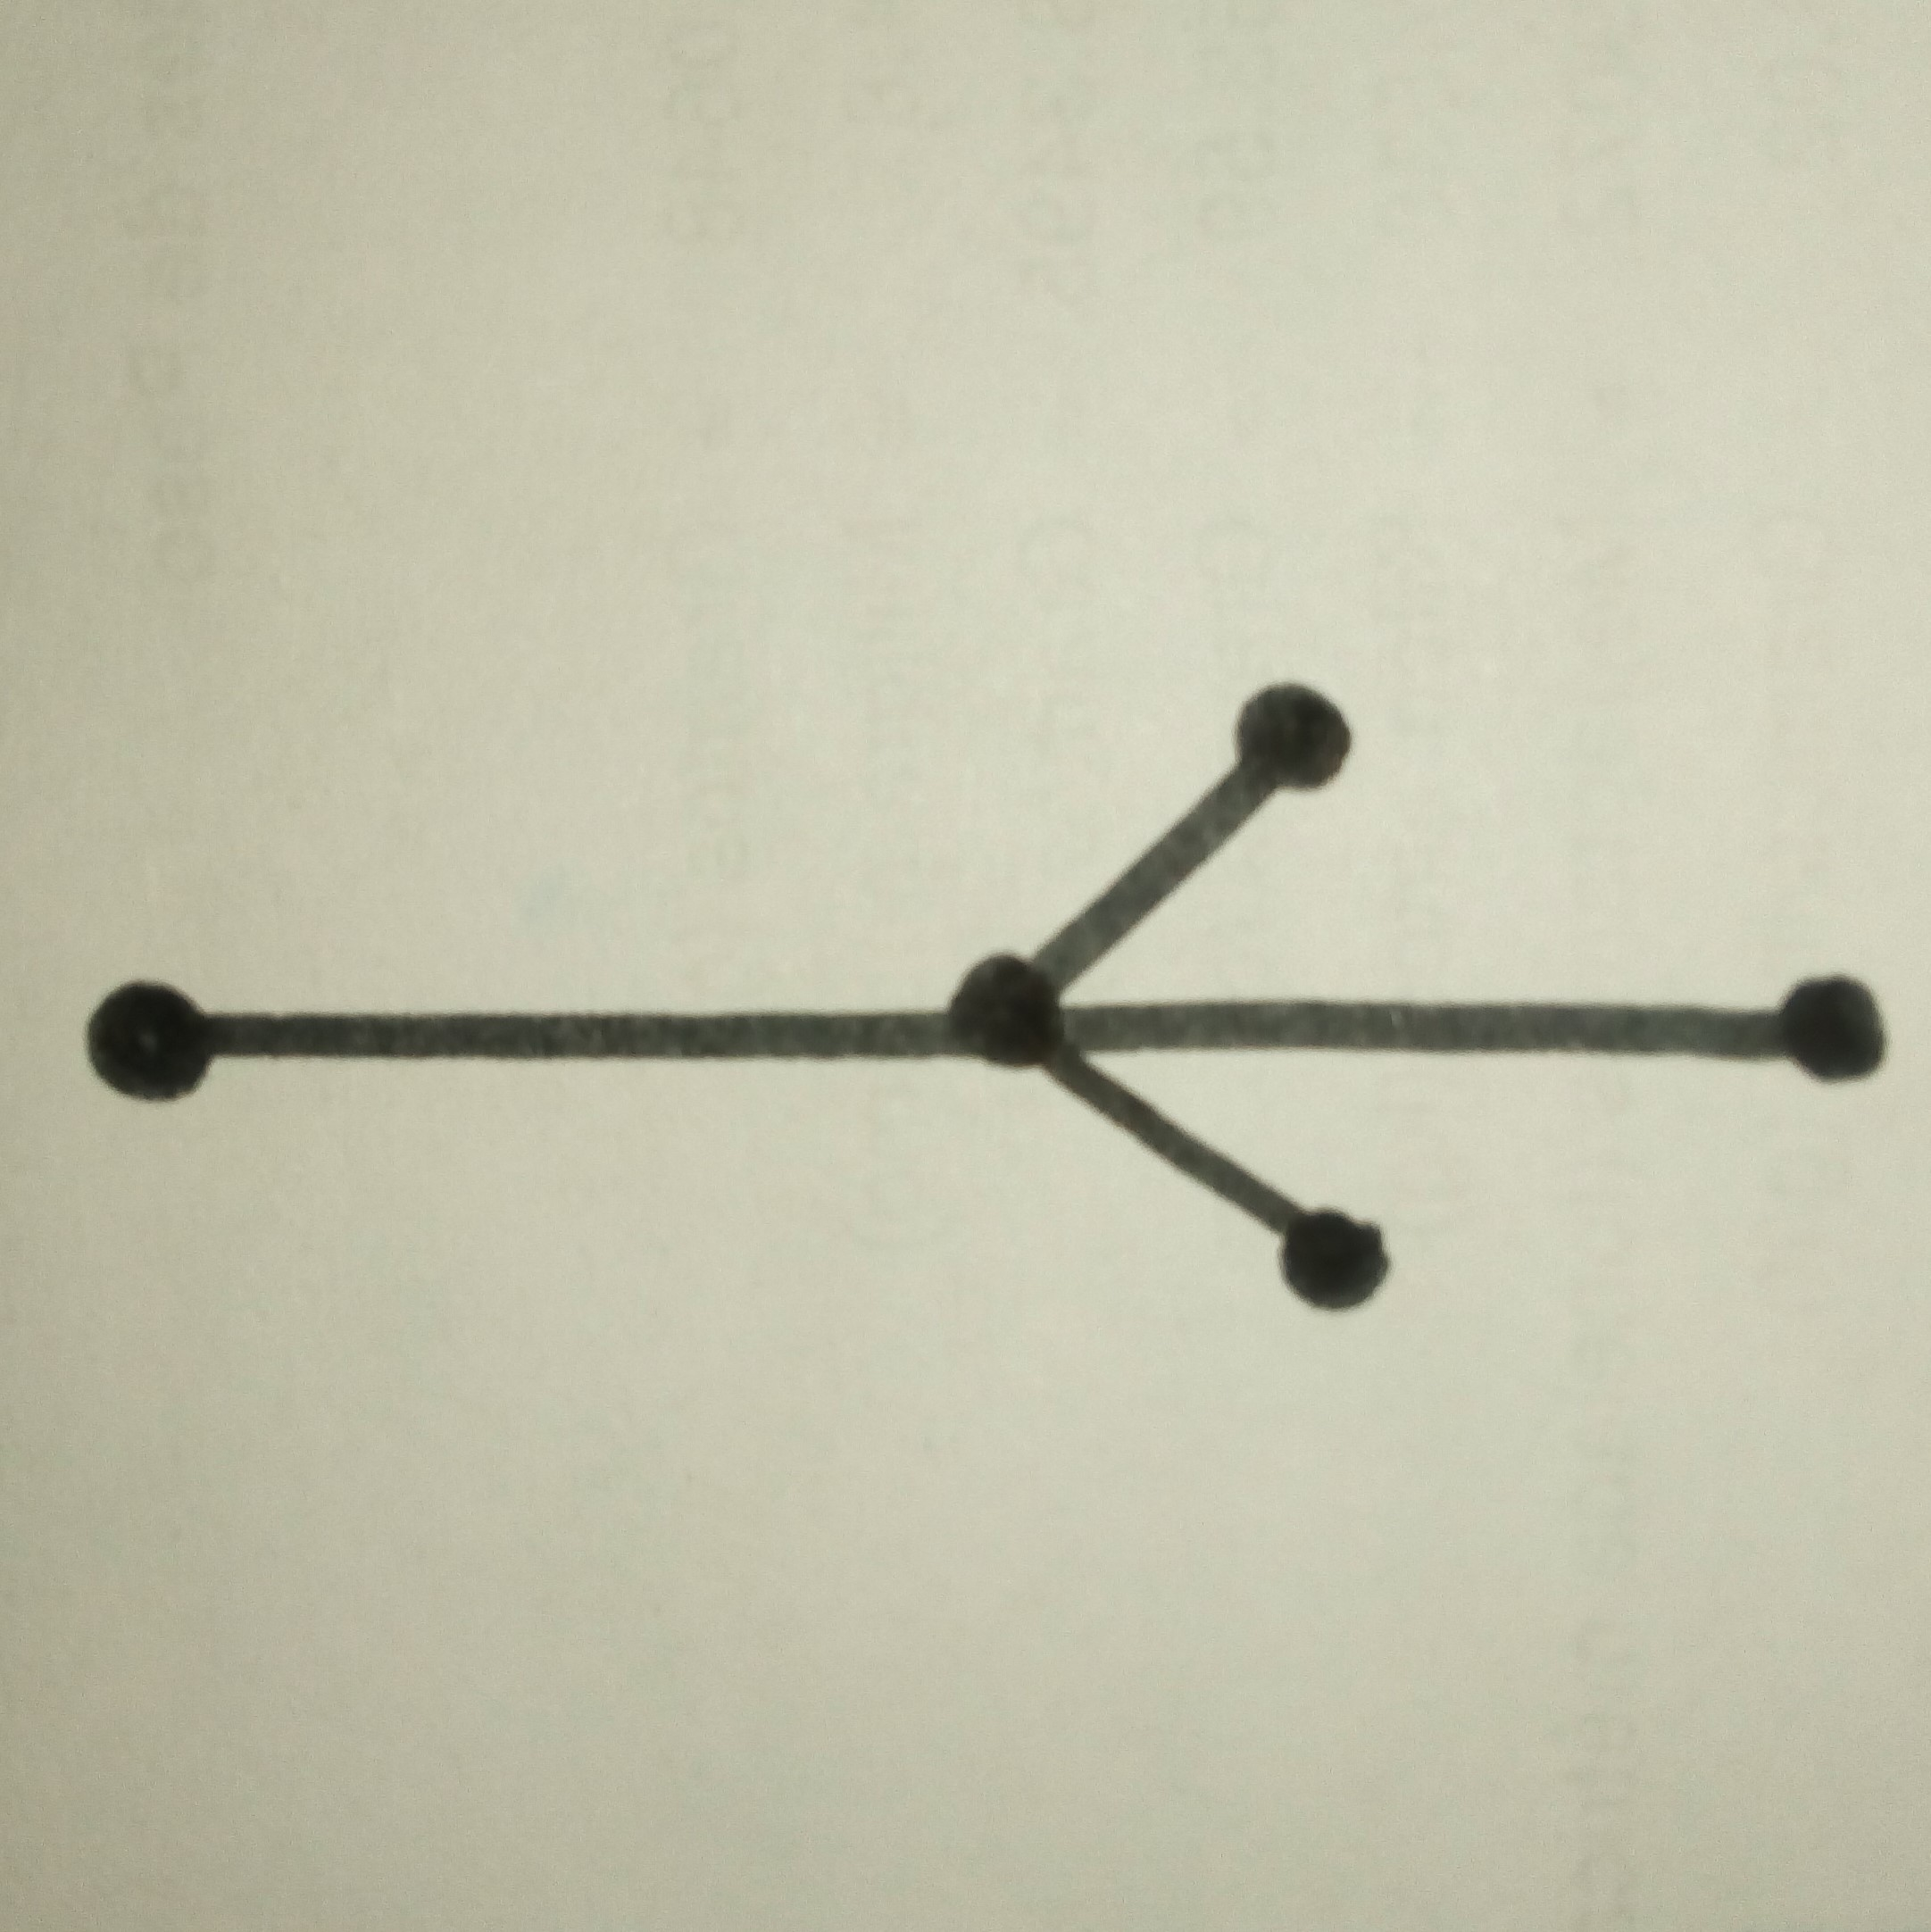
\includegraphics[scale=.05]{imagenes/9.jpg}
\end{center}
\begin{center}
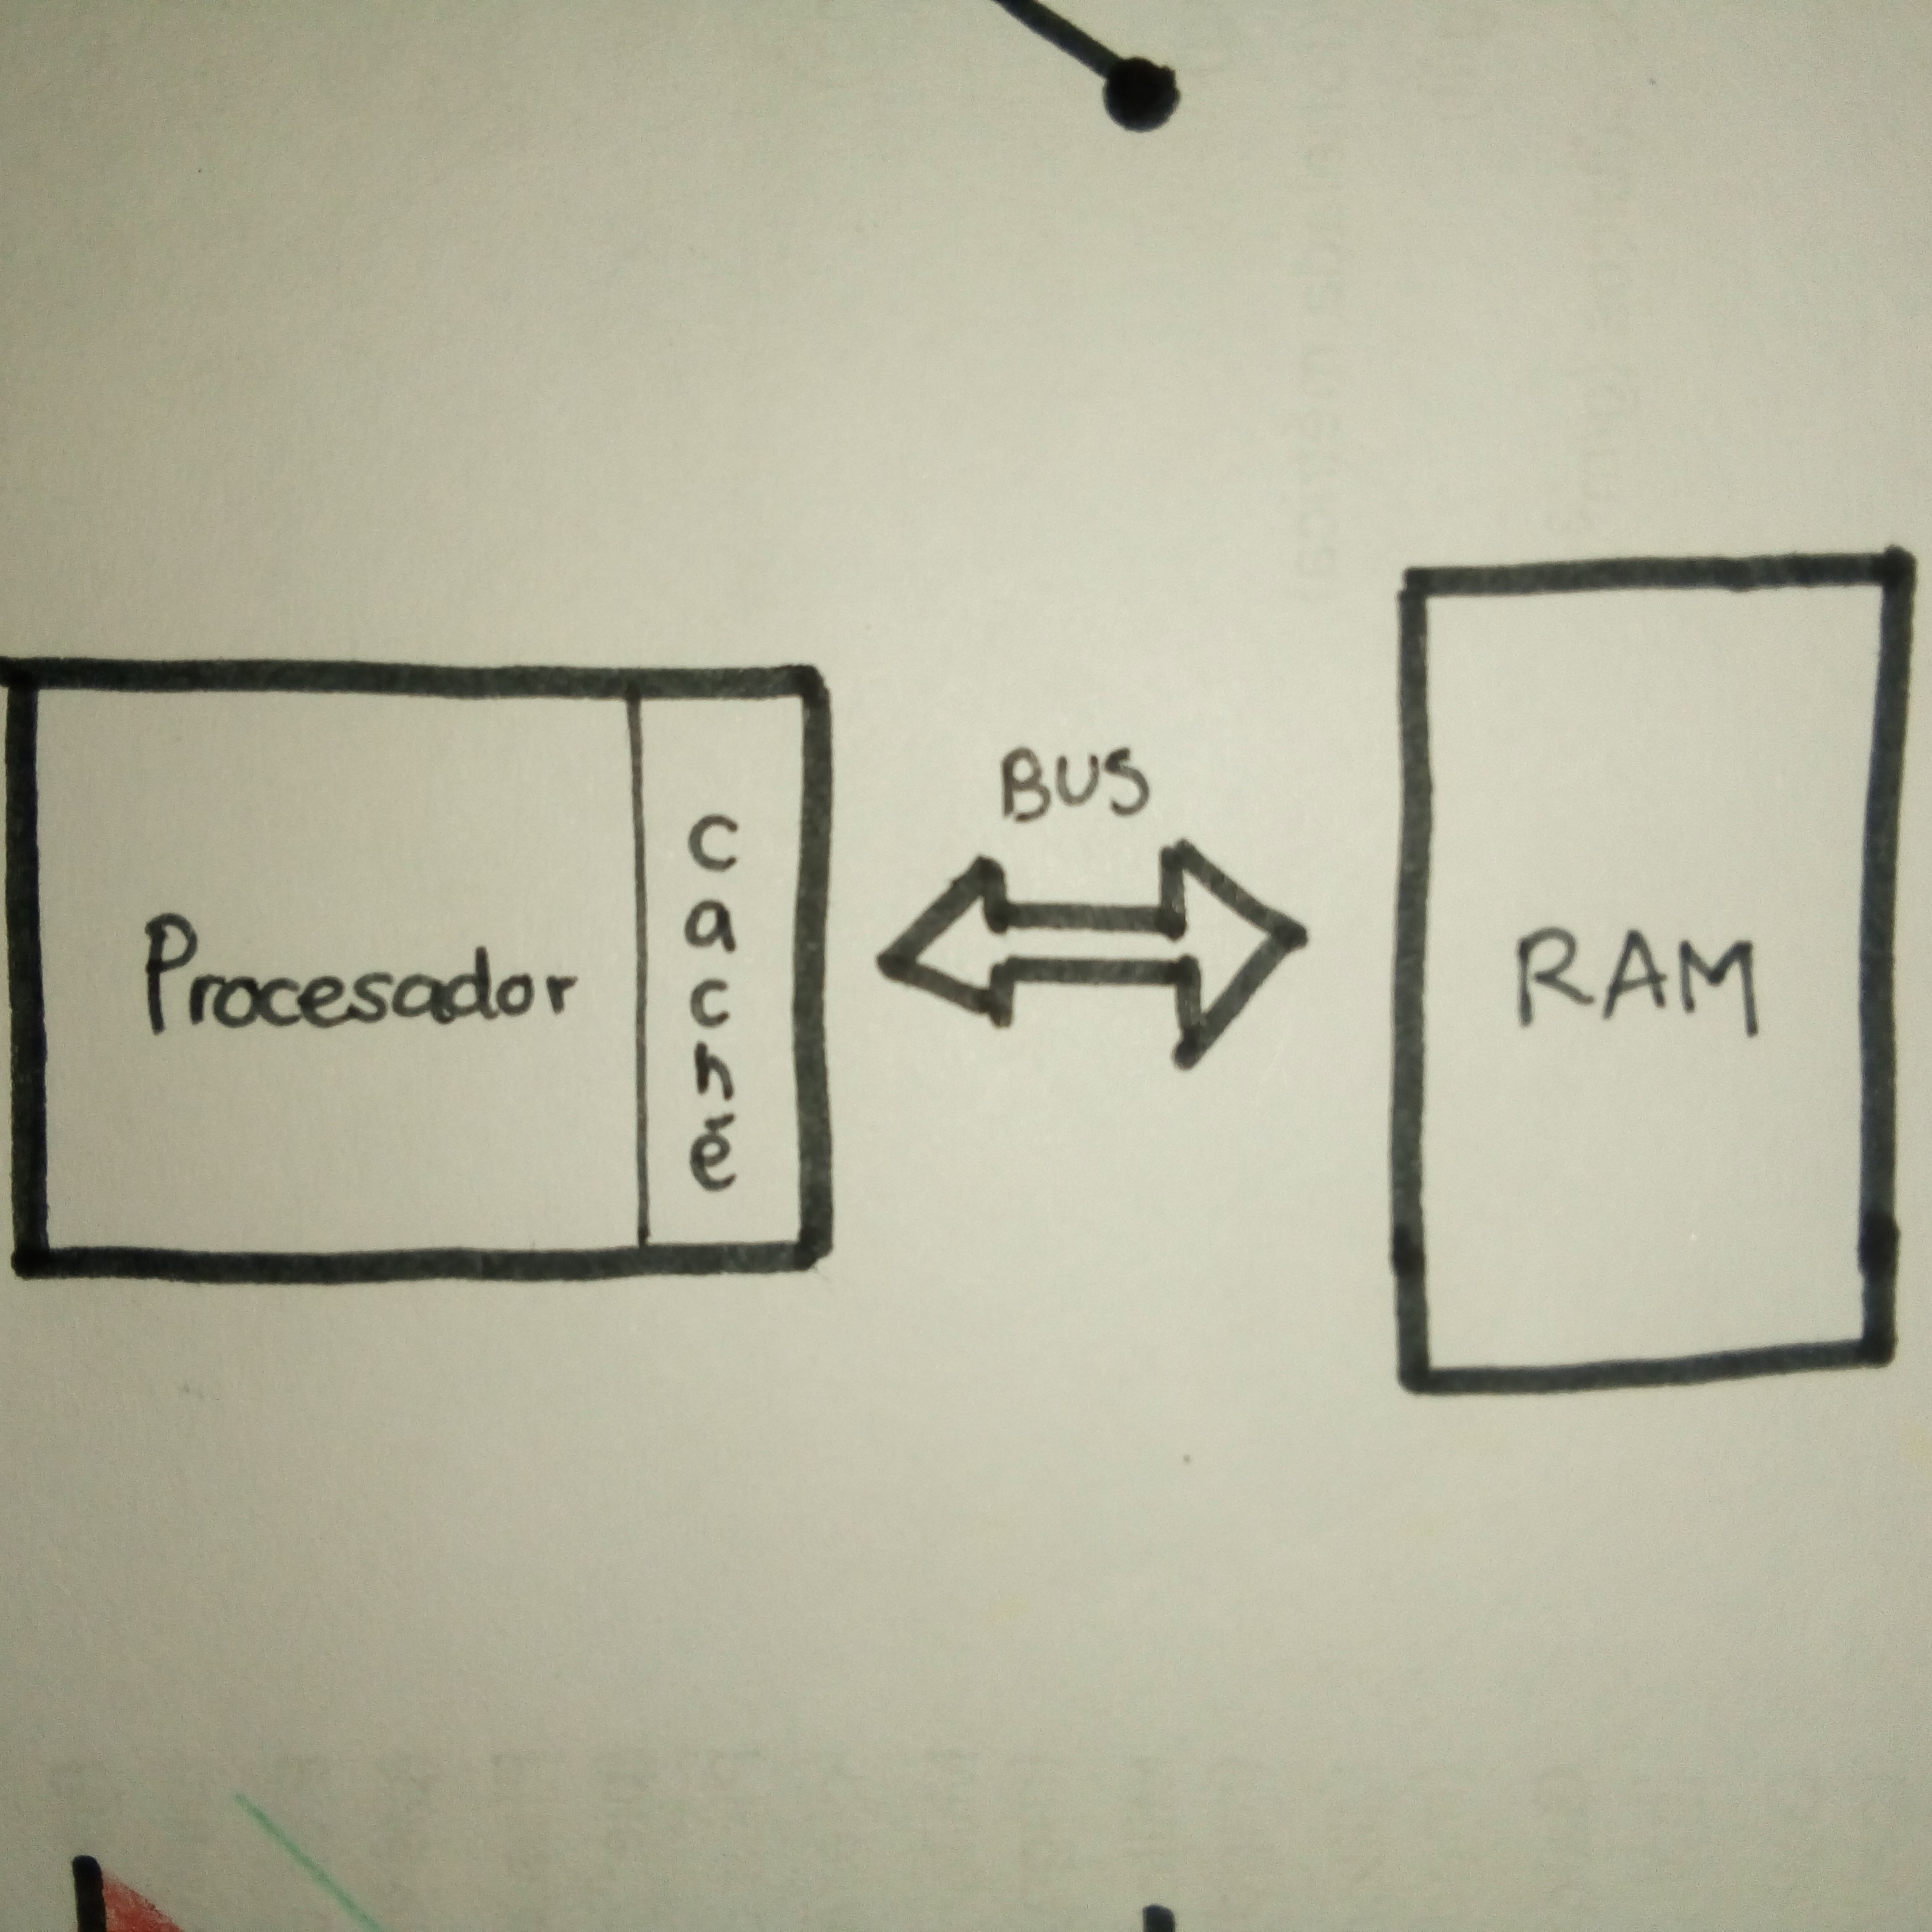
\includegraphics[scale=.05]{imagenes/10.jpg}
\end{center}
\subsection{Memoria cache}
Por ejemplo la memoria cache es mucho m\'as r\'apida que la memoria RAM.\\
Es m\'as f\'acil acceder por renglones que por columnas, en una matriz.\\
LAs lineas de la cache hacen que el sistema sea más eficiente (En una linea de 64 bytes).\\
$A\cdot V \rightarrow rapido$\\
$A^T\cdot V\rightarrow Lento$

\section{Adaptaci\'on para matrices dispersas}
Antes es importante recordar el tamaño de algunos tipos de datos y las equivalencias existentes entre tamaños de datos. 
\begin{tabular}{| c | c |}
\hline
Tipo de dato & Cantidad de bytes \\
\hline
int & 4 \\
double & 8\\
\hline
\end{tabular}
\subsection{Matriz sin reducci\'on o con ancho de banda completa}
Para calcular el espacio que ocupa una matriz de tamaño $m \times n$:
\begin{displaymath}
n\times m\times (cantidad\quad bytes*)
\end{displaymath}
*(depende el tipo de dato) 
\subsubsection{Matriz sim\'etrica}
Solo se toma la mitad de ancho de banda.\\
Este m\'etodo puede ser tambien m\'as lento debido a la busqueda por columnas pero usa menos espacio de memoria y es m\'as rapida que la eliminaci\'on Gaussiana con banda.
\begin{displaymath}
s=(m+1)/2
\end{displaymath}
\begin{displaymath}
n \times s
\end{displaymath}
donde $(m+1)$ siempre es impar.
\begin{center}
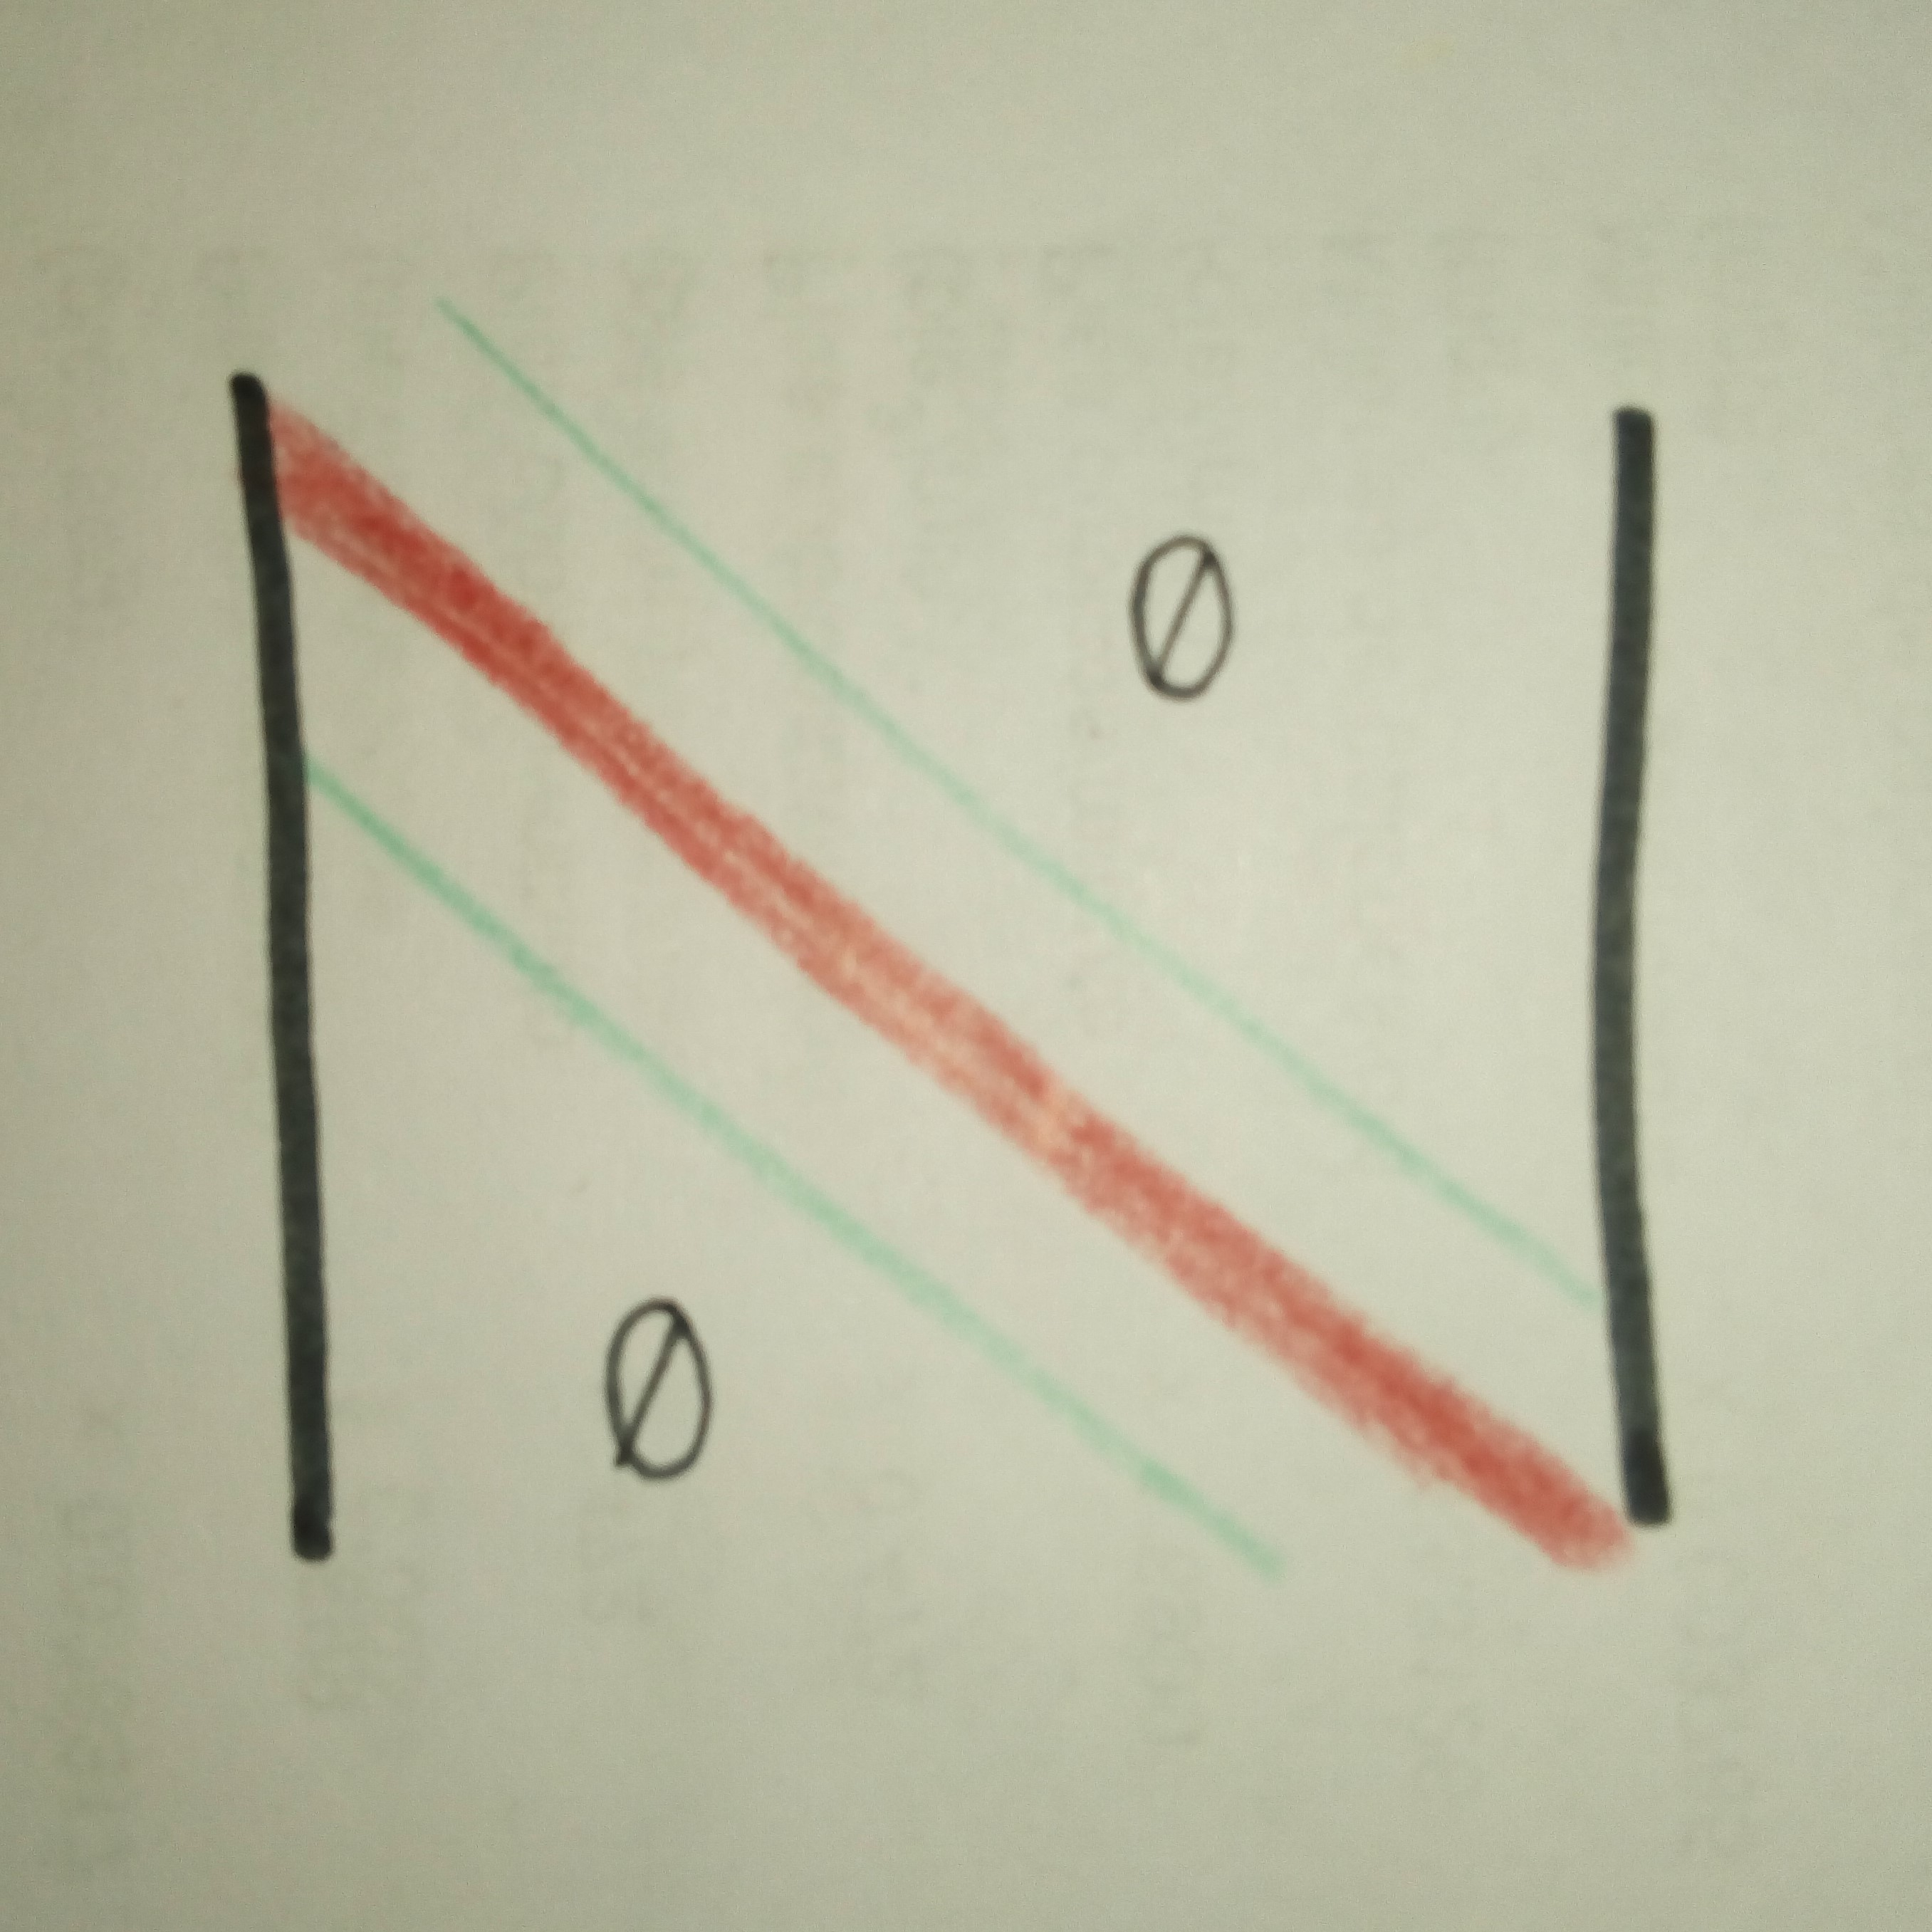
\includegraphics[scale=.05]{imagenes/11.jpg}
\end{center}
\subsection{M\'etodo para matrices skyline}
Depende del tipo de m\'etodo se elegira la manera de almacenarlas ya sea por trianguci\'on superior, inferior.\\
No es tan \'util para m\'etodos iterativos, usa menos espacio en metodos directos y es m\'as util para m\'etodos directos y sim\'etricos. Es espacio total utilizado esta dado por:
\subsection{M\'etodo de compresi\'on por remglones}
\begin{displaymath}
nnz(8+4)+n\times 4
\end{displaymath} 
donde $nnz$ es el n\'umero de elementos distintos de cero.\\
Los m\'etodos directos primero hacen factorizaci\'on simbolica para ver que ceros de la matriz original son llenados.
\begin{center}
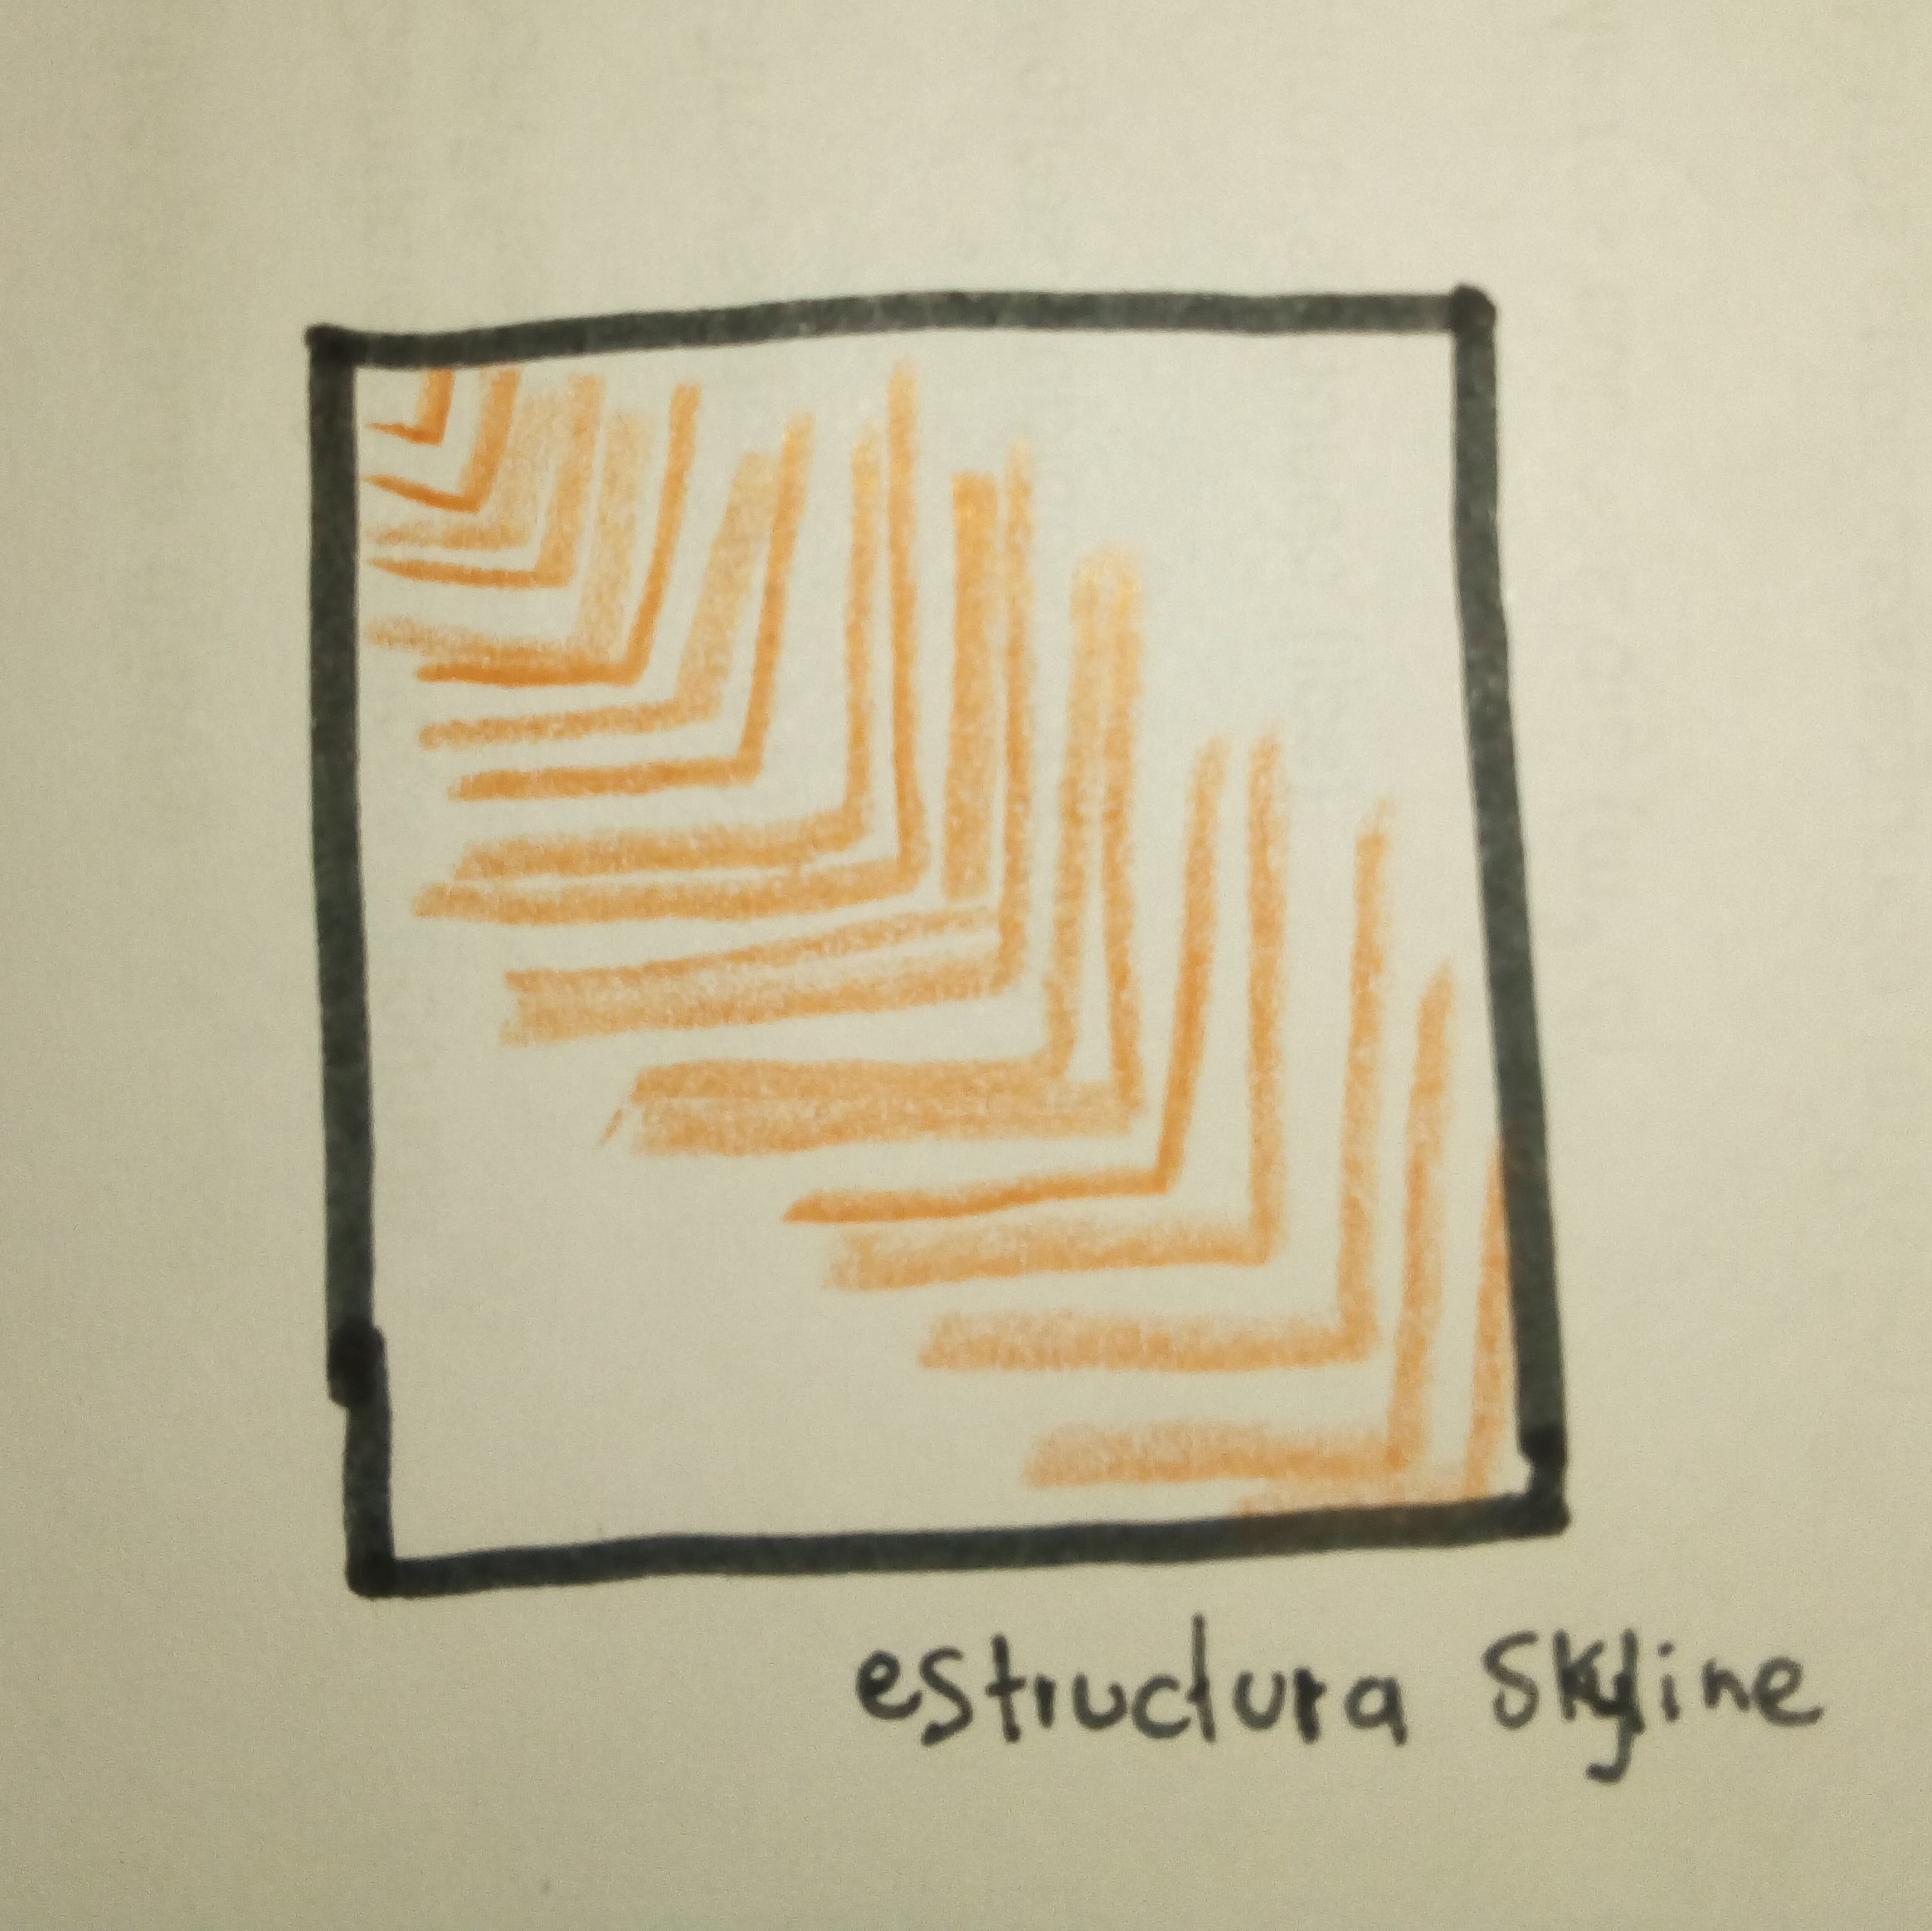
\includegraphics[scale=.05]{imagenes/12.jpg}
\end{center}

\section{Resumen de cápitulo}
Es recomendable utilizar una tolerancia de $1e^{-12}$ para resolver sistemas.\\
Los m\'etodos con banda completa, tarden mucho en converger al resultado.\\
Los m\'etodos con precondicionamiento CPS es mejor usarlos primero.\\
Es de mucha utilidad estimar primero la complejidad de los m\'etodos directos que es matriz$\cdot$vector, operacionalemente car. 
Muy importante es que los esquemas de almacenamiento matrices de banda no simetricas y matrices de bandas simetricas, solo se pueden usar para m\'etodos de soluci\'on que no destruyan la simetr\'ia de la matriz. Cholesky, LDLT y los iterativos.\\
El m\'etodo de almacenamiento de la columna din\'amica (Skyline) es util para m\'etodos de factorizaci\'on y no es recomendable para m\'etodos iterativos, pero si para matrices sim\'etricas de modo que se almacene solo la triangulaci\'on inferior o superior 